% Name: Monopoly pricing
% Description: A monopolist produces where marginal revenue equals marginal cost and charges what demand will bear there, earning the profit rectangle and leaving a deadweight loss against the competitive outcome.
% Tags: monopoly, marginal revenue, marginal cost, deadweight loss, microeconomics

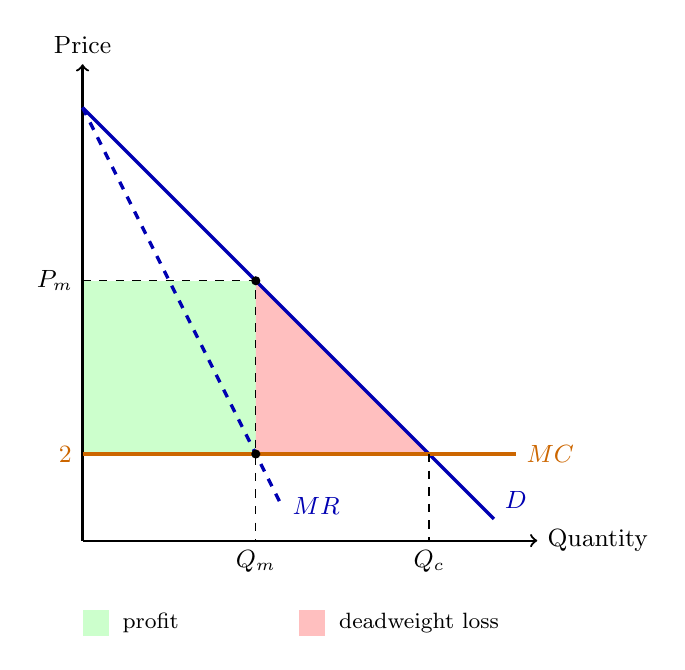
\begin{tikzpicture}[scale=0.55, every node/.style={font=\small}]
  % Demand P = 10 - Q, so MR = 10 - 2Q; with MC = 2, MR = MC at Q = 4 and P = 6, against Q = 8 under competition
  \fill[green!20] (0,2) rectangle (4,6);
  \fill[red!25] (4,6) -- (4,2) -- (8,2) -- cycle;
  \draw[->, thick] (0,0) -- (10.5,0) node[right] {Quantity};
  \draw[->, thick] (0,0) -- (0,11) node[above] {Price};
  \draw[very thick, blue!70!black] (0,10) -- (9.5,0.5) node[above right] {$D$};
  \draw[very thick, blue!70!black, dashed] (0,10) -- (4.6,0.8) node[right] {$MR$};
  \draw[very thick, orange!80!black] (0,2) node[left] {$2$} -- (10,2) node[right] {$MC$};
  \draw[dashed] (0,6) node[left] {$P_m$} -| (4,0) node[below] {$Q_m$};
  \draw[dashed] (8,2) -- (8,0) node[below] {$Q_c$};
  \fill (4,6) circle (3pt) (4,2) circle (3pt);
  % Swatches under the axis name the shaded areas
  \fill[green!20] (0,-2.2) rectangle ++(0.6,0.6);
  \node[anchor=west, font=\footnotesize] at (0.7,-1.9) {profit};
  \fill[red!25] (5,-2.2) rectangle ++(0.6,0.6);
  \node[anchor=west, font=\footnotesize] at (5.7,-1.9) {deadweight loss};
\end{tikzpicture}
